\section{Program Logic for Location Virtualization}
\label{sec:logic}
% The predicate gen_heap_interp.
\newcommand{\gammaPred}{\delta}

\newcommand{\sumwalkabs}[3]{
  \ownGhost\gammaPred{\authfrag{\singletonMap{#1}{(#2, #3)}}}
}
\newcommand{\ptableabswalk}[1]{\mathcal{A}\textsf{bsPTableWalk}(#1)}
\newcommand{\ptablestore}{\theta}
Our reasoning principles are shaped around understanding the following perspectives on the vritual-memory abstraction:
\begin{enumerate}
\item \textit{logical representation of addressing}: we present physical memory addressing as separation-logic points-to relations.
\item \textit{sharing}: a bag of physical pages are reached through a set of physical page-table (L4-L1 page-tables) acceses that are shared amongst different virtual addresses. This sharing imposes constraints on giving a definition to the virtual-address in terms of physical (L4-L1) page-table memory accesses
\item \textit{context-agnostic-resources}: each virtual address is valid under a certain address-space, but it does not represent this \textit{knowledge} on its address-space. 
\item \textit{address-spaces as modal-contexts}: we call these context-agnostic resources (virtual-address pointstos) as \textit{context-resource}, and the context identfied by a unique \textit{namespace}, and  defining the truth for these context resources as \text{modal-context}
\item \textit{updating inter/intra address-spaces}: we present logical abstractions to enable allocating/updating pages in the existence of \textit{sharing}  
\item \textit{address-space switch as changing the "World" of truth}: switching from one address-space to another logically becomes introduction of \textit{context-resources} to the \textit{modal-context} under which they are valid, and loading \textit{context-resources} that are valid under the \textit{currently} loaded address-space
\end{enumerate}
Based on these perspectives, we coneptualize truth on an address-space through the contingency it exhibits: \textit{assertion P holds on this address-space indexed by its roots address}. Therefore, as a first step, we lift standard bi proposition to be indexed with $\mathcal{W}_{64}$ as shown in Figure \ref{fig:vprop}, and, most notably, all abstractions we explain in this section as part of our custom-tailored address-space logic are type $\textsf{vProp }\Sigma$.
\begin{figure}[!ht]
\[
\begin{array}{cl}
\textsf{vProp } \Sigma \; : \; \textsf{bi} \; \stackrel{def}{=} \mathcal{W}_{64} \rightarrow_{\textsf{b}} \textsf{iPropI } \Sigma
\end{array}
\]
\caption{$\textsf{vProp }\Sigma$: Root-Address Indexed Address-Space Proposition}
  \label{fig:vprop}
\end{figure}
%\subsection{Machine State under Address Translation}
%\label{sec:selectedinstrsemantics}
%Althought we give the complete set of operational semantics rule in \sref{appendix:movops}, It is worth building the intuition on the the way some of these rules bahave in the context of address translation. In fact $\readlval\maddr{\storememstar\crval}\locsf$ is unfoled into multiple physical memory lookups for the final page address retrieval -- i.e. address translation traversal as shown in Figure \ref{fig:pagetables}:
%\begin{itemize}
%\item top-level-address translation: with the given root address (64-bit $\crval$) of the address space, performs the address translation, handling the first level (to get the PML4 entry) itself. The next level table address is computed with the fetched PML4 offset value which exhibits itself as 9-bit offset in $\kw{maddr}$. \mytodo{iso: put move}
%\item translating from PML4 entry: performs the second level of address translation, to retrieve starting at the PML4 table entry, and interprets the PML4 entry that references a Page-Directory-Pointer Table (PDPT). We obtain the PDPT offset which exhibits itself as 9 bit offset in $\kw{maddr}$ to obtain the address of the next level page directory table (PDT) \mytodo{iso: put move}
%\item translating from PD entry: performs the third level of address translation, to retrieve starting at the PDP table entry, and interprets a PDPTE that references a PD table. Likewise, we obtain the PD offset which exhibits itself as 9 bit offset in $\kw{maddr}$ to obtain the address of the next level page directory table (PT) \mytodo{iso:put move }
%\item translate from PT entry: performs final level of address translation, starting from the PT entry, with a given 12 bit page offset, we can compute the physical address referencing $\locsf$ \mytodo{ismo: put mov}
%\end{itemize}
\subsection{Points-To Assertions}
\label{sec:pointsto}
We abstract physical memory addressing and registers naming with well-known separation logic assertion \textit{points-to} assertions.
\begin{enumerate}
\item Physical address points-to, $\pfpointsto\locsf\vpts\qfrac\ppts$
\item Register points-to, $\pfpointsto\rg\rv\qfrac\rpts$
\end{enumerate}
\paragraph{Register points-to} The assertion $\pfpointsto\rg\rv\rpts\qfrac$ ensures the ownership of the register $\rg$ naming the register value $\rv$. The fraction $\qfrac$ with value 1 asserts the unique ownership of the register mapping, and grants update permission on it, otherwise, any value $0 < \qfrac <1$ represents partial ownership granting readonly permission on the mapping.
\paragraph{Physical-Memory points-to} Our physical memory points-to relation in Figure \ref{fig:physicalpointsto} for a page table entry (e.g. \textsf{PDE} in Figure \ref{fig:pagetables}) abstracts masking -- $|^{52}$ for frame for and $|^{12}$ for offset -- through logical nested maps.  
\begin{figure}[!ht]
\[
\begin{array}{cl}
\pfpointsto\locsf\vpts\qfrac\ppts \stackrel{def}{=} & \nfpointsto{\mask\locsf\ft\generalentry}{\mask\locsf\tw\generalentry}\vpts\qfrac\naddr
\end{array}
\]
\caption{Physical Points-to with Nested Masking}
  \label{fig:physicalpointsto}
\end{figure}
Given the definition of physical page-pointsto assertion and the root address of virtual-address space kept in the control register \textsf{CR3} as shown in Figure \ref{fig:pagetable},  one can build the physical address-translation for a virtual address (e.g. \textsf{va}) via abstracting the L4-L1 table traversal as the following:
\begin{itemize}
  \item Page Map Level-4 Translation (L4): Address translation, handling the first level (to get the PML4E entry) itself by calculating the offset (\textsf{CR3}$|^{12}$) and frame (PML4E$|^{52}$) via masking with the root address space address currently stored in \textsf{CR3}.
    \[ \begin{array}{l}
      \hbox{(\TirNameStyle{{L4translate}})} \quad
      \exists \entryf \ldotp \nfpointsto{\mask\vaddr\ft\crthree}{\mask\vaddr\tw\crthree}\entryf\qfracfotsss\naddr
      \end{array}
      \]
  \item Page Directory Pointer Level Translation (L3): Performs the second level of address translation via interpreting, in other words masking, the PML4 entry (PML4E$|^{52}$) to retrieve the starting address of a page-directory-pointer-table and the offset ( (PML4E$|^{9}$)) to the entry
    \[\begin{array}{l}
    \hbox{(\TirNameStyle{{L3translate}})} \quad
    \exists \entrytr \ldotp \nfpointsto{\mask\vaddr\ft\entryf}{\mask\vaddr\tw\entryf}\entrytr\qfracfotss\naddr
    \end{array}
    \]
  \item Page Directory Table Level Translation (L2):  Performs the third level of address translation by retrieving the starting address at the PD table (PDPE$|^{52}$), and interprets a PDPE ($|^{9}$) that references the PD table entry.
    \[ \begin{array}{l}
            \hbox{(\TirNameStyle{{L2translate}})} \quad 
       \exists \entrytw \ldotp \nfpointsto{\mask\vaddr\ft\entrytr}{\mask\vaddr\tw\entrytr}\entrytw\qfracfots\naddr
      \end{array}
      \]
  \item Page Table Level Translation (L1):
    \[ \begin{array}{l}
      \hbox{(\TirNameStyle{{L1translate}})} \quad
      \exists \entryo \ldotp \nfpointsto{\mask\vaddr\ft\entrytw}{\mask\vaddr\tw\entrytw}\entryo\qfracfot\naddr
      \end{array}
      \]
  \item Page Address Level Translation
    \[ \begin{array}{l}
      \hbox{(\TirNameStyle{{PageLebelAccess}})} \quad
      \exists \vpage \ldotp \nfpointsto{\mask\vaddr\ft\entryo}{\mask\vaddr\tw\entryo}\vpage\qfracone\naddr
      \end{array}
      \]
    
\end{itemize}
\begin{remark}[A Strong Definition for Virtual Memory Addressing]
  \label{rem:strongvmem}
  One could give a naive logical definition to the virtual mememory addressing as conjuctions of each level translation (Figure \fref{fig:strongvirtualpointsto}). The very first assurance our logical constructions need to be able assert is the \textit{existence} of the page table walk. Our naive attempt shown in Figure \ref{figure:strongvirtualpointsto}, we see that a virtual address with a certain fractional permissions at each level of the page-table walk gives us sound assurance of the path existence reaching to a page table entry, consequently, with a full-ownership of page address, we can obtain and update the value mapped value at this physical page address through our virtual memory address. 

\begin{figure*}
  \[
  \begin{array}{l}
\begin{array}{l}
  \vaddr\mapsto_{\textsf{t}}\{\textsf{q}\}\vpage \stackrel{def}{=} \lambda \crthree.\\
  \exists_{\entryf \;, \entrytr \;, \entrytw \;,\entryo} \ldotp 

  \ulcorner \textsf{aligned } \vaddr \urcorner \ast  \\
  \textsf{L}_{4}\_\textsf{L}_{1}\_\textsf{PointsTo}(\crthree,\entryf,\entrytr,\entrytw,\entryo)\\
   \nfpointsto{\mask\vaddr\ft\entryo}{\mask\vaddr\tw\entryo}\vpage\qfracone\naddr 
\end{array} \\

\textsf{where   }\textsf{L}_{4}\_\textsf{L}_{1}\_\textsf{PointsTo}(\vaddr,\crthree,\entryf,\entrytr,\entrytw,\entryo) \stackrel{\triangle}{=} \\
 \qquad\qquad \nfpointsto{\mask\vaddr\ft\crthree}{\mask\vaddr\tw\crthree}\entryf\qfracfotsss\naddr \ast \\ 
 \qquad\qquad  \nfpointsto{\mask\vaddr\ft\entryf}{\mask\vaddr\tw\entryf}\entrytr\qfracfotss\naddr  \ast  \\
  \qquad\qquad \nfpointsto{\mask\vaddr\ft\entrytr}{\mask\vaddr\tw\entrytr}\entrytw\qfracfots\naddr \ast \\
  \qquad\qquad \nfpointsto{\mask\vaddr\ft\entrytw}{\mask\vaddr\tw\entrytw}\entryo\qfracfot\naddr 
   \end{array}
\]
\caption{A Strong Virtual Points-to Relation}
\todo[inline]{These fractions aren't quite right (though I see you added the variance between levels), I can walk you through in our meeting tomorrow.}
  \label{fig:strongvirtualpointsto}
\end{figure*}
\end{remark}
%then we reach to a physical page addr (e.g. \textsf{pa}) 
%\[  \paddr\mapsto_{\textsf{a}}\{1\}\vsome \ast \nfpointsto{\mask\vaddr\ft\entryo}{\mask\vaddr\tw\entryo}\vpage\qfrac\naddr \]

  \subsection{Aliasing/Sharing Physical Pages}
  \label{sec:sharingpages}  
  One might have already observed that the virtual points-to definition shown in Figure \ref{fig:strongvirtualpointsto} is too strong to specify virtual memory operations updating a page table entry. To speak more concretely, the fractional permissions on the page-table-walk assertion ($textsf{L}_{4}\_\textsf{L}_{1}\_\textsf{PointsTo}$ in Figure \ref{fig:strongvirtualpointsto}) \textit{only} assure the existence of the certain number of mappings -- 512 at each level -- abstracting virtual address translations, and updating any of these mappings would make the other mappings, address translations sharing the page table mappings. Therefore, we need to have logical abstractions ensuring sound updates to the page-table entries in the existence of sharing.
  
 One possible approach is to abstract away the physical page-table-walk pointsto ($\textsf{L}_{4}\_\textsf{L}_{1}\_\textsf{PointsTo}$ in Figure \ref{fig:strongvirtualpointsto}) from the virtual pointsto relation via replacing it with read-only abstract map entries -- a ghost (abstract) map entry per \textsf{L}$_4$\_\textsf{L}$_{1}$ mappings -- which can be used as a resource ($ \sumwalkabs\vaddr\qfrac\paddr$) whose ownership ensures that the virtual address ($\vaddr$) is mapped to a page (referenced by $\paddr$) ,and as a token to access to the physical page-table-walk pointsto (\textsf{L}$_4$\_\textsf{L}$_{1}$) stored in an address-space invariant ($\mathcal{I}$\textsf{ASpace} in Figure \ref{fig:peraspaceinvariant}). We use \textsf{Iris}'s authorative ghost-map logical machinery
\[\mathcal{A}\textsf{bsPTableWalk} \stackrel{\triangle}{=} \textsc{Auth} (\; \mathcal{W}_{64} \;\rightarrow_{\textrm{fin}} \;  (\mathcal{W}_{64} \; \rightarrow_{\textrm{fin}}\;  (\textsc{Frac }, \mathord{+}) \times (\textsc{Agree } \Loc,\mathord{=}) ))\]
to realize these reasoning principles ($\mathcal{A}\textsf{bsPTableWalk}$).
\begin{remark}[Exchanging Page-Table-Walk-Summarization Mappings (Tokens) with Physical Page-Table-Walk Pointstos ]
  $\mathcal{A}\textsf{PTableWalk}$'s fragmental-ownership represents an individual key-value pair (per-virtual-address) which can be handled as a \textit{look-up} resource for an individual virtual address.
  To build more intuition, we can think of the use-case \textit{unmapping-pages} as collecting the fragmental map pairs, e.g. $\sumwalkabs\vaddr\qfrac\paddr$, from collecting the assertions, removing them from the ghost map, and then updating the page tables.
  Critically, physical full ownership ($\ownGhost\gammaPred{\authfull{\ptableabswalk\ptablestore}}$) of the page tables, as a \textit{singleton resource}, lives in the central invariant keeping physical-page-table pointstos per-virtual address translation.
  With this mechanism we can separate the virtual-to-physical translation from the physical memory involved, and consequently
  \begin{itemize}
  \item virtual pointsto assertions, whose definition is shown in Figure \ref{fig:virtualpointstosharing}, can refer to their physical memory assertions representing their page-address translation in the physical-page-tables ($\textsf{L}_{4}\_\textsf{L}_{1}\_\textsf{PointsTo}$) which reside in the address-space invariant ($\mathcal{I}$\textsf{ASpace} in Figure \ref{fig:peraspaceinvariant}) using individual key-value pair, i.e. instances of ($\sumwalkabs\vaddr\qfrac\paddr$)
  \item unlike the case in the strong virtual-pointsto relation in Figure \ref{fig:strongvirtualpointsto}, physical-page-table-walk pointsto assertions ($\textsf{L}_{4}\_\textsf{L}_{1}\_\textsf{PointsTo}$) for all virtual addresses are moved into the address-space invariant ($\mathcal{I}$\textsf{ASpace} in Figure \ref{fig:peraspaceinvariant}), and resides with authorative ownership of $\mathcal{A}\textsf{PTableWalk}$ ($\ownGhost\gammaPred{\authfull{\ptableabswalk\ptablestore}}$) which respects all entries of the abstract virtual-address translation mappings ($\sumwalkabs\vaddr\qfrac\paddr$).
    \end{itemize}
\end{remark}
\begin{figure*}
\[
\begin{array}{l}
    \vaddr\mapsto_{\textsf{v}}\{\textsf{q}\}\vpage \stackrel{\triangle}{=} 
  \exists \entryo \ldotp 
  \sumwalkabs\vaddr\qfrac\paddr \ast 
   \nfpointsto{\mask\vaddr\ft\entryo}{\mask\vaddr\tw\entryo}\vpage\qfracone\naddr
\end{array}
\]
\caption{Virtual-Pointsto for Sharing Pages}
  \label{fig:virtualpointstosharing}
\end{figure*}
%\subsection{Address-Space Abstraction}
%\label{sec:aspacemodal}

Then, once we want to outline the distribution of the facts per-address, as we see it pictorially  in Figure \ref{fig:logicaladdrspace}, the outline is composed of the following aspects:
\begin{enumerate}
\item a global address space invariant (solid round square labelled as $\mathcal{I}$\textsf{ASpace} in Figure \ref{fig:peraspaceinvariant}) asserting the authorative ownership (i.e. update capability), $\ownGhost\gammaPred{\authfull{\ptableabswalk\ptablestore}}$, of the ghost map -- shown as solid-round-head arrow to $\mathcal{A}\textsf{PTableWalk}$ Figure \ref{fig:logicaladdrspace}
\item per-virtual-pointsto relation ((cutted round square labelled as \textsf{Virtual PointsTo} in Figure \ref{fig:peraspaceinvariant})) asserting the fragmental ownership of the ghost map, $\sumwalkabs\vaddr\qfrac\paddr$ \textit{represents} the fragmental-ownership (cutted-diamond-head arrow) of $\mathcal{A}\textsf{PTableWalk}$
\item for each ghost page-table-walk mapping,  $\sumwalkabs\vaddr\qfrac\paddr$, there exists one shared persistent invariant (shown as double-ended solid arrow 1 to N)
  \[\textsf{L}_{4}\_\textsf{L}_{1}\_\textsf{PointsTo}(\crthree,\entryf,\entrytr,\entrytw,\entryo)\]
\end{enumerate}

\begin{figure}
   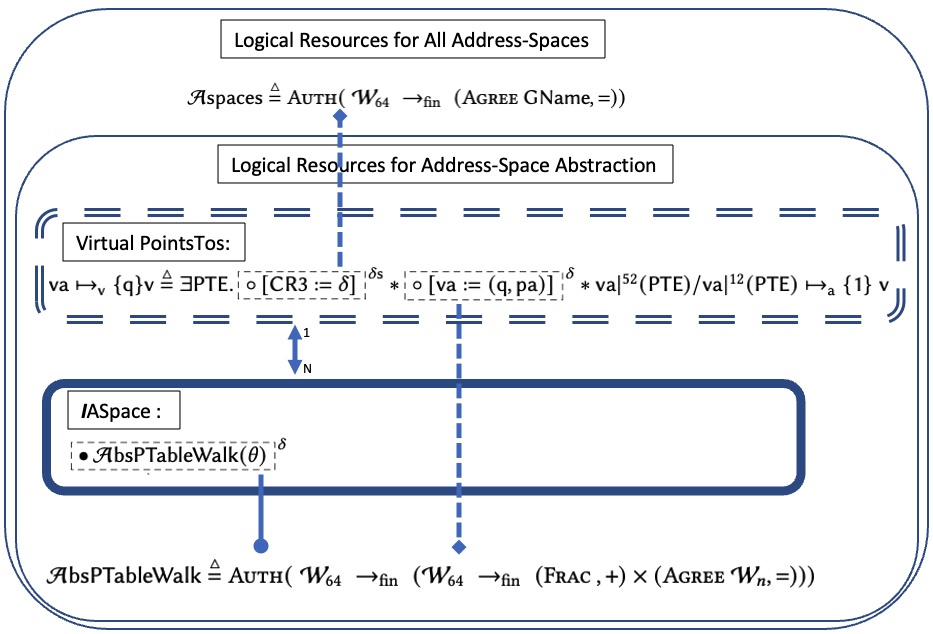
\includegraphics[width=0.75\columnwidth]{logical_addr_space.png}
  \caption{Logical Resources of Address-Space Abstraction}
  \label{fig:logicaladdrspace}
  \end{figure}
    \subsubsection{Global Per-Address-Space Invariant}
    \label{sec:peraspaceinvariant}
    Virtual points-to assertions would need to be defined in terms of physical points-to assertions and hardware-specific address translation assertions for mapped virtual addresses ($\textsf{L}_{4}\_\textsf{L}_{1}\_\textsf{PointsTo}(\crthree,\entryf,\entrytr,\entrytw,\entryo)$ in Figure \ref{fig:peraspaceinvariant}). For each virtual address \textit{mapped} with a physical page table entry, abstracted with ghost mappings ($\sumwalkabs\vaddr\qfrac\paddr$) in virtul-pointsto relations as shown in Figure \ref{fig:virtualpointstosharing}), there exsits a physical page table walk.  
    \[ \bigast{(\vaddr, \entryo)\in \ptablestore}{\exists\;(\entryf\;,\entrytr\;,\entrytw)\ldotp \textsf{L}_{4}\_\textsf{L}_{1}\_\textsf{PointsTo}(\vaddr,\crthree,\entryf,\entrytr,\entrytw,\entryo)} \]
    By separating the virtual-points Overlapping address spaces — both shared data, and shared page tables
which may see updates — can be coordinated with protocols to ensure those updates preserve
address space invariants.
\begin{figure*}
\[
\begin{array}{l}
  \mathcal{I}\textsf{ASpace} \stackrel{\triangle}{=} \lambda \; \crthree \ldotp
  \exists\;\gammaPred \;\ldotp\; \ownGhost\gammaPred{\authfull{\ptableabswalk\ptablestore}} \ast \\
  \bigast{(\vaddr, \entryo)\in \ptablestore}{\exists\;(\entryf\;,\entrytr\;,\entrytw)\ldotp \textsf{L}_{4}\_\textsf{L}_{1}\_\textsf{PointsTo}(\vaddr,\crthree,\entryf,\entrytr,\entrytw,\entryo)}
\end{array}
\]
\caption{Global Address-Space Invariant}
  \label{fig:peraspaceinvariant}
\end{figure*}
\subsection{Address-Space Management}
\label{sec:aspacemanagement}
With the reasoning principles introduced for the essential resource of address spaces, i.e. virtual memory addresses, now we can ...
% \item abstractions shaped-around address-space switch where all virtual pointsto assertions happen to be true in a certain address space, i.e. the truth on address virtualization is indexed by CPUs page table register ($\crthree$ for x86-64), and we present modal reasoning principles for updating $\crthree$ (switching from the current address space to another) 
\subsubsection{Address-Space Modality}
\label{sec:aspacemodalist}
The truth on an address space, exhibits itself as a contingent truth: a location virtualization assertion (a virtual points-to in \ref{fig:virtualpointstosharing}),  happens to valid in the \textit{current world} (in the current address space), and switching address spaces pulls information out of one \textit{world} into the “current view” of memory, and leaves other assertions true relative to the previous address space.
\begin{figure}
   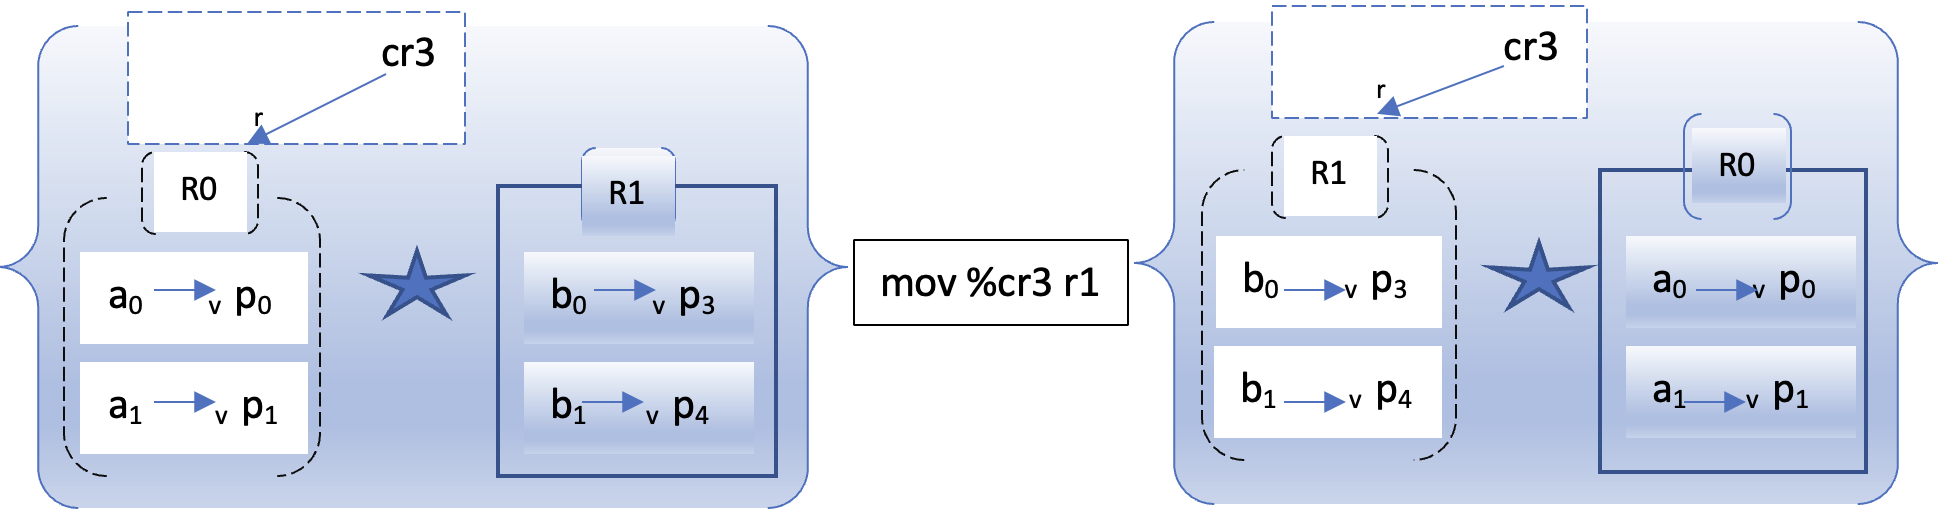
\includegraphics[width=\columnwidth]{addr_space_switch.png}
  \caption{Loading an Address-Space into the Current Memory View}
  \label{fig:addrswitch}
  \end{figure}
Therefore, an address-space, as an abstraction, can be treated as naming the memory state as a modal frame and the choice of page table root as a world in Kripke-style semantics. Not suprisingly, transition between two address-spaces, then, can be just an entailment relation \textit{alternating} the \textit{named-state} against the address-space invariant ($\mathcal{I}\textsf{ASpace}$ in Figure \ref{fig:peraspaceinvariant}). 
\[
  \begin{array}{l}
    \hbox{(\TirNameStyle{ModalAddressSpace})} \\ \qquad
         [r](P)  \;\stackrel{\triangle}{=}  (\mathcal{W}_{64} \rightarrow_{\textsf{b}} \textsf{uPredI} (\textsf{iResUR} \;\Sigma)) \rightarrow_{\textsf{b}} \textsf{uPredI } \_ := \lambda \textsf{P},\; \textsf{P r}. 
  \end{array}
\]
Being inspired by what hybrid logic \ref{} calls a satisfaction operator, which evaluates the truth of a predicate in a named alternative state (here, address space), we give a modal definition describing the truth of assertions for the resources (i.e. virtual pointsto relations) inside the address space. Ignoring the predicate types for a while, $[r]P$ in Definition $\hbox{(\TirNameStyle{ModalAddressSpace})}$, indicates that $P$ holds in the virtual address space rooted at $r$, the truth ($P$) on an address-space is indexed by the root page-table address $r$ of the address-space. In the rest of this section, we explain the structural aspects -- the modal resource context of address space modality -- , and how we lift the interaction of address-space modality with the ambient logic, i.e. separation logic as an entailment for specifying \textit{address-space-switch}.  
\paragraph{Modal Resource Context}
\label{sec:resourcecontext}
When we pick up a certain contingency, which is \textit{"a certain virtual-pointsto facts whose validity is indexed by the root address of an address space"}for address space modality, we, in fact, make our choice around some logical resources for which we care about reasoning, which is virtual pointsto relation shown in Figure \ref{fig:virtualpointstosharing}. In other words, our modality definition is the logical virtual pointsto resources: introduction/elimination of logical virtual pointsto resources are the ones essential to the reasoning capabilities the address space modality provides, i.e. validity of virtual addresses under/out of modality -- resources under/out of \textit{modal resource context}.

The choice of resource defining the modal context already exhibits itself as a reasoning principle (Figure \ref{fig:modalcontextinvariance}) in which we can intro/eliminate any resource that is not virtual pointsto into/from modal context without dischargin any obligation. We can use this entailment for  \todo[inline,color=red]{Ask Colin}.
  \[
  \begin{array}{l}
\hbox{(\TirNameStyle{ModalContextInvariance})} \qquad
 [r](Q \ast \ell \mapsto_{\textsf{p}} \vpage)  \;\vdash [r](Q) \ast \ell \mapsto_{\textsf{p}} \vpage 
  \end{array}
  \]
\begin{remark}[The Choice of Modal Context Definition as a Pattern of Verification Context]
  \label{remark:pattern}
  By choosing the contingency and what defines the modal contex, we simply introduce 
  \begin{enumerate}
  \item the pattern of what the essential abstraction (e.g. address spaces) we care about to do verification for is
  \item how a modal context (e.g. a address-space modality $[r]P$), logically, draws the attention to the certain facts in the interest of reasoning (e.g. virtual pointsto relations in the current address-space in Figure \ref{fig:virtualpointstosharing})
  \item and, offloads the burden of individual bookkeeping of these facts (e.g. virtual pointsto relations per address-space) under different context (e.g. virtual pointsto relations in other address-spaces) via utilizing the \textit{summarization} aspect of the contingency it represents (e.g. other virtual pointsto relations are valid under other certain address-space page-table root addresseses).  
  \end{enumerate}
\end{remark}
\paragraph{Interaction}
\label{sec:interaction}
So far, we have just mentioned the structural properties of our modal definition (Remark \ref{remark:pattern}), and what inherent entailments (Rule \hbox{(\TirNameStyle{ModalContextInvariance})}) these properties provide. However, all these structural aspects of using the address-space modality ($[r]P$) considers the fixed index ($r$) of on the truth $P$. From the client's perspective, structural properties of the modal abstraction mainly constitutes the modal frame with summarizing the facts for one another address-space under the address-space modality roughly as it is in the following spec
\[
\{ \crthree \mapsto_{r} r0 \ast \textsf{va1} \mapsto_{v} \textsf{v}_1 \ast \textsf{va2} \mapsto_{v} \textsf{v}_2 \ast \textsf{va3} \mapsto_{v} \textsf{v}_3 \ast [r1]\;P \}
\]
where we see the \textit{current address-space} rooted at $r0$ is loaded into the  \textit{current-view} of the memory with its resources ($ \textsf{va1} \mapsto_{v} \textsf{v}_1 \ast \textsf{va2} \mapsto_{v} \textsf{v}_2 \ast \textsf{va3} \mapsto_{v} \textsf{v}_3$), and framed by the address-space rooted at $r1$ with resources $P$. 
Now, we need to a rule capturing the notion that switching the address spaces by pulling the resources ($P$) out of the one under modality into the \textit{“current view”} of memory, and leaves other assertions true relative to the previous address space (the one rooted at $r0$). To do so, we need to have a proof rule for the instruction (\lstinline|mov_ctl|) updating the $\crthree$.

\subsection{Considering Hoare Doubles in the Context of Switching Address-Space}
An important subtlety arises with supporting \lstinline|mov|s into \lstinline|%cr3|. Consider the hypothetical rule:
\begin{mathpar}
\inferrule[Broken]{ }{
  \{P \ast cr3\mapsto_{r} \;r_1 \ast r \mapsto_{r} \;r_2 \ast [r_2](Q)\}
  \texttt{mov}~\texttt{\%cr3},~r%\lstinline|mov %cr3, r| 
  \{[r_1](P) \ast cr3 \mapsto_{r} r_2 \ast r \mapsto_{r} r_2 \ast Q\}
}
\end{mathpar}
This rule captures the intuitive change of address space in a Hoare triple, rather than double, form. The problem with this is that it interacts quite poorly with the traditional frame rule and the modal flavor of virtual points-to assertions:
\begin{mathpar}
  \inferrule*[right=Frame]{
    \inferrule*[right=Broken]{ }{
    \{\mathsf{emp} \ast cr3 \mapsto_{r} r_1 \ast r\mapsto_{r} r_2 \ast [r_2](Q)\}
    \texttt{mov}~\texttt{\%cr3},~r%\lstinline|mov %cr3, r| 
    \{[r_1](\mathsf{emp}) \ast cr3 \mapsto_{r} r_1 \ast r \mapsto_{r} r_2 \ast Q\}
    }
  }{
    \{a\mapsto_\mathsf{v} x \ast \mathsf{emp} \ast cr3\mapsto_{r}r_1 \ast r \mapsto_{r}r_2 \ast [r_2](Q)\}
    \texttt{mov}~\texttt{\%cr3},~r%\lstinline|mov %cr3, r| 
    \{a\mapsto_\mathsf{v} x \ast [r_1](\mathsf{emp}) \ast cr3 \mapsto_{r} r_1 \ast r \mapsto_{r} r_2 \ast Q\}
  }
\end{mathpar}
Notice that both the precondition and postcondition assert that $a\mapsto_\mathsf{v} x$ in the current address space, but we have no basis for concluding that address translation is preserved by the change of address space. So this derivation clearly leads to an unsound conclusion. This suggestss that the traditional frame rule and the Hoare triple presentation of the change-of-address-space rule cannot soundly coexist in the same system.
The heart of the problem is that while updating \lstinline|cr3| is \emph{physically} local, it globally changes the interpretation of virtual addresses. So it is simply unsound to frame around \lstinline|cr3| updates.

Switching to Hoare doubles resolves this problem because an under-appreciated subtlety of Hoare doubles is that typically \emph{there is no frame rule}. Instead each verification essentially includes a local frame that it passes to the next instructions (think continuation-passing style), giving each overall rule a \emph{global} (rather than local) precondition. For most rules this is not that important, but it does permit rules that have global effects on their preconditions.

This is then how we justify our actual rule for \lstinline|cr3| updates:
\begin{mathpar}
\inferrule[ChangeAddressSpace]{
  \{[r_1](P) \ast cr3 \mapsto_{r} r_2 \ast r \mapsto_{r} r_2 \ast Q\}\overline{is}
}{
  \{P \ast cr3 \mapsto_{r} r_1 \ast r \mapsto_{r} r_2 \ast [r_2](Q)\}
  \texttt{mov}~\texttt{\%cr3},~r;\;\overline{is}
  %\lstinline|mov %cr3, r| 
}
\end{mathpar}
Because the precondition on this rule is global, we avoid issues with framing.

If we wanted to consider a frame rule that would work for this logic, we could consider:
\begin{mathpar}
  \inferrule[Cr3Frame]{
    \{P\ast cr3=v\}\;C\;\{ Q \ast cr3=v\}
  }{
    \{R\ast P\ast cr3=v\}\;C\;\{ R \ast Q \ast cr3=v\}
  }
\end{mathpar}
By demanding that \lstinline|cr3| be held constant (or rather, at least restored to its original value) we could frame almost traditionally. In particular, this rule would work with framing around calls that might lead to address space switches, such as calling blocking operations in the kernel.

Readers familiar with dynamic frames~\cite{parkinson2011relationship} might find it useful to notice that a different perspective on this matter is that virtual points-to assertions are self-stable \emph{except} for changes in \lstinline|cr3|, so framing would then naturally require other means of holding \lstinline|cr3| constant (or saving and restoring it).
Virtual points-to assertions could be made self-stable by also giving them partial ownership over \lstinline|cr3| assertions, but this would require explicitly plumbing that ownership from \emph{all} assertions back to any place an address space change might occur; this would seem to be a far graver loss of modularity than this extra quirk in framing discussions.
\begin{figure}
\begin{mathpar}
\inferrule[WriteToRegFromReg]{
  \{P \ast r_d \mapsto_{r} \textsf{rvs} \ast r_s \mapsto_{r}\{q\} \textsf{ rvs} \}\;\overline{ is}
}{
  \{P \ast r_d \mapsto_{r} \textsf{rvd} \ast r_s \mapsto_{r}\{q\} \textsf{ rvs} \}
  \textsf{ mov}~\textsf{r}_d,~\textsf{r}_s;\;\overline{is}
  %\lstinline|mov %cr3, r| 
}
\\
\inferrule[WriteToMemFromReg]{
  \{P \ast r_s \mapsto_{r}\{q\}  \textsf{rvs} \ast \textsf{cr3} \mapsto_{r} \textsf{cr3val}  \ast r_a \mapsto_{r} \{q\} \textsf{ vaddr} \ast (\textsf{vaddr} \mapsto_{\textsf{t}} \textsf{v})\;\textsf{cr3val} \}\;\overline{ is}  
}{
  \{P \ast r_s \mapsto_{r}\{q\}  \textsf{rvs} \ast \textsf{cr3} \mapsto_{r} \textsf{cr3val}  \ast r_a \mapsto_{r}\{q\} \textsf{ vaddr} \ast (\textsf{vaddr} \mapsto_{\textsf{t}} \textsf{rvs})\;\textsf{cr3val} \}
  \textsf{ mov}~\textsf{r}_a,~\textsf{r}_s;\;\overline{is}
}
\\
\inferrule[WriteToRegFromMem]{
  \{P \ast r_d \mapsto_{r}  \textsf{v} \ast \textsf{cr3} \mapsto_{r} \textsf{cr3val}  \ast r_a \mapsto_{r} \{q\} \textsf{ vaddr} \ast (\textsf{vaddr} \mapsto_{\textsf{t}} \textsf{v})\;\textsf{cr3val} \}\;\overline{is}
}{
  \{P \ast r_d \mapsto_{r}  \textsf{rvd} \ast \textsf{cr3} \mapsto_{r} \textsf{cr3val}  \ast r_a \mapsto_{r} \{q\} \textsf{ vaddr} \ast (\textsf{vaddr} \mapsto_{\textsf{t}} \textsf{v})\;\textsf{cr3val} \}
  \textsf{mov}~\textsf{r}_d,~\textsf{r}_a;\;\overline{is}
}
\\
\inferrule[WriteToRegCtlFromReg]{
  \{P \ast r_s \mapsto_{r}\{q\}  \textsf{ rvs} \ast \textsf{cr3} \mapsto_{r} \textsf{rvs}  \}\overline{is}
}{
  \{P \ast r_s \mapsto_{r}\{q\}  \textsf{ rvs} \ast \textsf{cr3} \mapsto_{r} \textsf{cr3val}  \}
  \textsf{mov}~\textsf{cr3},~r_s;\;\overline{is}
  %\lstinline|mov %cr3, r| 
}
\end{mathpar}
\caption{Selected Reasoning Rules for ..}
\label{fig:wpdamd}
\end{figure}
\paragraph{Register To Memory}
\paragraph{Memory To Register}
\paragraph{Register To Register}
\todo[inline,color=red]{STOP HERE}
